\documentclass[11pt]{article}

% --- Geometry ---
\usepackage[margin=1.1in]{geometry}

% --- Fonts (modern sans-serif body; Latin Modern Sans is the only widely
% available Helvetica-adjacent option in this TeX install) ---
\usepackage[T1]{fontenc}
\usepackage{lmodern}
\renewcommand{\familydefault}{\sfdefault}
\usepackage{microtype}    % refined character protrusion / font expansion

% --- Tables / figures ---
\usepackage{booktabs}
\usepackage{array}
\usepackage[table,dvipsnames]{xcolor}
\usepackage{graphicx}
\usepackage{float}
\usepackage{caption}
\captionsetup{font=small,labelfont=bf,skip=4pt}

% --- Math ---
\usepackage{amsmath}

% --- Spacing ---
\usepackage{parskip}
\setlength{\parskip}{0.55\baselineskip}
\linespread{1.07}

% --- Section headings (modest emphasis, similar size to body) ---
\usepackage{titlesec}
\titleformat{\section}{\large\bfseries}{\thesection}{0.6em}{}
\titleformat{\subsection}{\normalsize\bfseries}{\thesubsection}{0.6em}{}
\titlespacing*{\section}{0pt}{1.4em}{0.4em}
\titlespacing*{\subsection}{0pt}{0.9em}{0.3em}

% --- Hyperlinks ---
\usepackage[hypertexnames=false]{hyperref}
\hypersetup{
    colorlinks=true,
    linkcolor=teal!60!black,
    citecolor=teal!60!black,
    urlcolor=blue!60!black,
}

% --- Title ---
\title{TIBU Data Quality Audit}
\author{Jenny Zhao\\\small Wellesley College \and Erez Yoeli\\\small MIT Sloan School of Management}
\date{}

\begin{document}

\maketitle
\tableofcontents
\newpage

\section{Overview}

This document presents a data quality audit (DQA) of TIBU, Kenya's national electronic TB reporting system. The audit was conducted in the context of the Keheala Study 2 randomized controlled trial (see \href{https://www.medrxiv.org/content/10.64898/2026.02.11.26346015v1}{medRxiv:2026.02.11.26346015v1}), but its scope is TIBU-specific and the findings stand independently of the trial results.

TIBU is a paper-to-digital reporting system: clinic staff record treatment data on the paper TB register at the point of care, and TB clerks subsequently transcribe entries from the paper register into TIBU. We therefore treat the paper register as the ground truth; a TIBU--paper discrepancy reflects a gap or error on the transcription side rather than at point of care.

The TIBU extract available for this audit covers patients registered between April 2018 and December 2019 ($N = 119{,}653$ nationwide), with treatment outcomes recorded through late 2021. The long outcome window reflects standard TB treatment duration: roughly six months for drug-sensitive disease and up to 18--24 months for multidrug-resistant (MDR) disease. A paper-registry audit was conducted across study clinics in multiple waves beginning in late 2018; the latest outcome dates captured by the audit fall in mid-2020, implying the final wave ran into the second half of 2020. The audit yielded $3{,}645$ records, of which $3{,}370$ could be matched to a corresponding TIBU record and form the basis of the DQA (see \S\ref{sec:matching} on the matching procedure). Tables~\ref{tbl:patient_char} and~\ref{tbl:outcomes} characterize three nested cohorts: all patients registered in TIBU during the study period, patients at study clinics in TIBU, and the subset of study-clinic patients whose records were audited.

The audit covers two categories of recording error. The primary analysis (\S\ref{sec:outcome_errors}) compares the \textbf{treatment-outcome field} as recorded in TIBU against the paper registry, quantifying outcome misclassification. A complementary analysis of errors in the \textbf{date fields} (registration date, outcome date) is in progress and will be added as a subsequent section.

For the outcome analysis, patients recorded as transferred out in TIBU---including those assigned the MT4 code, used when drug resistance is discovered mid-treatment and the patient is referred to a drug-resistant TB program---are excluded, as a transfer is not an auditable final outcome. Records where the paper registry has no outcome are also excluded, as the audit requires ground truth. Among the remaining patients, three types of outcome discrepancy are distinguished:

\begin{itemize}
\itemsep0pt
    \item \textbf{False positive} in the digital record (a Type~I error): TIBU records a successful outcome (treatment completion or cure) but the paper registry records a failure (death, treatment failure, or loss to follow-up). Clinically: TIBU \emph{overstates} the program's success.
    \item \textbf{False negative} in the digital record (a Type~II error): TIBU records a failure while the paper registry records success. Clinically: TIBU \emph{understates} the program's success.
    \item \textbf{Missing in TIBU}: TIBU contains no outcome but the paper registry does. This is distinct from loss-to-follow-up, which is itself a recorded outcome: ``missing in TIBU'' means the clinic did record an outcome on paper, but the TIBU entry was never created or never finalized.
\end{itemize}
The cross-tabulation in Table~\ref{tbl:crosstab} maps the full distribution of these discrepancies across outcome categories. Subsequent subsections of \S\ref{sec:outcome_errors} then ask, in order, \emph{when} errors occurred (a smoothed time-series of error rates over the study period), \emph{where} they occurred (clinic-level breakdowns by province, urbanicity, and size), and \emph{who} experienced them (patient-level breakdowns by sex, age, disease type, and HIV status); a multivariate counterpart of the where/who breakdowns appears in Appendix~\ref{sec:appendix_logit}.

\vspace{6pt}
\noindent\fbox{\begin{minipage}{\dimexpr\textwidth-2\fboxsep-2\fboxrule}
\vspace{2pt}
\textbf{Key findings.} Across 3,054 classifiable audit records: false-positive raw rate 1.0\%; false-negative rate 0.7\%; records missing from TIBU 3.8\%. The false-positive rate likely overstates true TIBU misclassification: $\sim 70\%$ of false-positive records appear to be audit-snapshot artifacts (paper was updated after the audit transcribed it; TIBU then reflected the revised outcome), and a date-direction sensitivity classification (\S\ref{sec:date_errors}) cuts the rate roughly in half (to $0.5\%$). False-negative and missing-in-TIBU rates are not affected by this caveat. The missing-in-TIBU rate is dominated by a COVID-era reporting gap ($\sim$15\% for treatment outcomes in 2020 Q1--Q2), concentrated at two clinics; outside that window, all three outcome-error rates are low and roughly flat across the study period.
\vspace{2pt}
\end{minipage}}
\vspace{6pt}

% =============================================================================
\section{Patient Characteristics}
% =============================================================================

Tables~\ref{tbl:patient_char} and~\ref{tbl:outcomes} describe the study
population across three cohorts: all patients registered in the TIBU electronic
system during the study period, patients at study clinics recorded in TIBU, and
the subset of study-clinic patients whose records were audited in the paper
registry DQA.

\renewcommand{\thetable}{1a}
\begin{table}[H]
    \centering
    \caption{Individual and disease characteristics across TIBU and paper registry cohorts.}
    \label{tbl:patient_char}
    \scriptsize{
\begin{tabular}{lrr|rr|rr}
\hline\hline \\[-8pt]
Characteristic & \multicolumn{4}{c}{Digital} & \multicolumn{2}{c}{Paper} \\
 & \multicolumn{2}{c}{\shortstack{All \\ (N=119,653)}} & \multicolumn{2}{c}{\shortstack{Study clinics \\ (N=14,962)}} & \multicolumn{2}{c}{\shortstack{Study clinics \\ (N=3,263)}} \\
 & $N$ & (\%) & $N$ & (\%) & $N$ & (\%) \\ \hline \\[-8pt]
\textit{Individual characteristics} & & & & & & \\
\quad Male & 75,597 & (63.2\%) & 9,514 & (63.6\%) & 2,037 & (64.5\%) \\
\quad Mean age (years) & 36.1 & & 34.4 & & 32.7 & \\
\rule{0pt}{14pt}\textit{Disease characteristics} & & & & & & \\
\quad Bacteriologically confirmed & 62,149 & (51.9\%) & 11,243 & (75.1\%) & 2,223 & (70.4\%) \\
\quad Drug resistant & 1,343 & (1.1\%) & 2 & (0.0\%) & 3 & (0.1\%) \\
\quad Extrapulmonary TB & 17,558 & (14.7\%) & 1,794 & (12.0\%) & 360 & (11.4\%) \\
\quad HIV coinfection & 32,077 & (26.8\%) & 3,981 & (26.9\%) & 717 & (23.2\%) \\
\quad Retreatment & 8,351 & (7.0\%) & 1,262 & (8.7\%) & 290 & (9.4\%) \\
\hline\hline
\end{tabular}}
\end{table}

\renewcommand{\thetable}{1b}
\begin{table}[H]
    \centering
    \caption{Treatment outcomes across TIBU and paper registry cohorts.}
    \label{tbl:outcomes}
    \scriptsize{
\begin{tabular}{lrr|rr|rr}
\hline\hline \\[-8pt]
Characteristic & \multicolumn{4}{c}{Digital} & \multicolumn{2}{c}{Paper} \\
 & \multicolumn{2}{c}{\shortstack{All \\ (N=119,653)}} & \multicolumn{2}{c}{\shortstack{Study clinics \\ (N=14,962)}} & \multicolumn{2}{c}{\shortstack{Study clinics \\ (N=3,263)}} \\
 & $N$ & (\%) & $N$ & (\%) & $N$ & (\%) \\ \hline \\[-8pt]
\textit{Outcomes} & & & & & & \\
\quad Cured & 25,399 & (21.2\%) & 6,757 & (45.2\%) & 1,114 & (34.1\%) \\
\quad Treatment completed & 31,719 & (26.5\%) & 6,637 & (44.4\%) & 1,468 & (45.0\%) \\
\quad Died & 4,911 & (4.1\%) & 765 & (5.1\%) & 181 & (5.5\%) \\
\quad Treatment failed & 382 & (0.3\%) & 123 & (0.8\%) & 34 & (1.0\%) \\
\quad Lost to follow-up & 3,594 & (3.0\%) & 680 & (4.5\%) & 125 & (3.8\%) \\
\quad Not completed & 47,184 & (39.4\%) & 0 & (0.0\%) & 87 & (2.7\%) \\
\quad Transfer out & 6,382 & (5.3\%) & 0 & (0.0\%) & 138 & (4.2\%) \\
\quad Not TB & 0 & (0.0\%) & 0 & (0.0\%) & 0 & (0.0\%) \\
\quad Missing & 82 & (0.1\%) & 0 & (0.0\%) & 116 & (3.6\%) \\
\hline\hline
\end{tabular}}
\end{table}
\setcounter{table}{1}
\renewcommand{\thetable}{\arabic{table}}

% =============================================================================
\section{Record Matching Procedure}
\label{sec:matching}
% =============================================================================

\textit{Placeholder --- details of the matching procedure (identifiers used, handling of near-duplicates, reasons for non-matches) are currently being confirmed with the Keheala data team and will be added in a subsequent revision. The headline figures are: $3{,}645$ audited paper records, of which $3{,}370$ ($92.5$\%) were matched to a TIBU entry; the remaining $275$ unmatched audit records are excluded from the DQA because no corresponding TIBU counterpart exists.}

% =============================================================================
\section{Outcome Errors}
\label{sec:outcome_errors}
% =============================================================================

\subsection{Crosstab of TIBU vs.\ Paper Registry Outcomes}

Table~\ref{tbl:crosstab} shows the full cross-tabulation of treatment outcomes
recorded in TIBU against outcomes recorded in the paper registry for all
matched patients ($N = 3{,}370$). Counts on the diagonal are concordant; off-diagonal cells are the discrepancies that drive the error rates reported in the subsequent tables. The shaded regions mark the false-positive (red), false-negative (green), and missing-in-TIBU (blue) partitions used throughout the document.

\begin{table}[H]
    \centering
    \caption{Cross-tabulation of treatment outcomes in TIBU vs.\ paper registry.}
    \label{tbl:crosstab}
    \resizebox{\textwidth}{!}{\newsavebox{\DQACrosstabBox}
\savebox{\DQACrosstabBox}{\scriptsize{
\begin{tabular}{l|rr|rr|rr|rr|rr|rr|rr|rr|r}
\hline \hline \\[-8pt]
Outcome in TIBU & \multicolumn{16}{c}{Treatment Outcome in Paper Registry} & Total\\
& \multicolumn{2}{c|}{Blank} & \multicolumn{2}{c|}{C} & \multicolumn{2}{c|}{D} & \multicolumn{2}{c|}{F} & \multicolumn{2}{c|}{LTFU} & \multicolumn{2}{c|}{NC} & \multicolumn{2}{c|}{TC} & \multicolumn{2}{c|}{TO} & \\ 
& $N$ & (\%) & $N$ & (\%) & $N$ & (\%) & $N$ & (\%) & $N$ & (\%) & $N$ & (\%) & $N$ & (\%) & $N$ & (\%) & \\ \hline \\[-8pt]
Blank & 82 & (76.6\%) & \textcolor{blue}{14} & \textcolor{blue}{(13.1\%)} & \textcolor{blue}{1} & \textcolor{blue}{(0.9\%)} & \textcolor{blue}{0} & \textcolor{blue}{(0.0\%)} & \textcolor{blue}{2} & \textcolor{blue}{(1.9\%)} & 0 & (0.0\%) & \textcolor{blue}{6} & \textcolor{blue}{(5.6\%)} & \textcolor{blue}{2} & \textcolor{blue}{(1.9\%)} & 107 \\
C & 41 & (3.6\%) & 995 & (87.0\%) & \textcolor{red}{1} & \textcolor{red}{(0.1\%)} & \textcolor{red}{3} & \textcolor{red}{(0.3\%)} & \textcolor{red}{7} & \textcolor{red}{(0.6\%)} & 0 & (0.0\%) & 55 & (4.8\%) & \textcolor{red}{42} & \textcolor{red}{(3.7\%)} & 1,144 \\
D & 4 & (2.2\%) & \textcolor{green!60!black}{2} & \textcolor{green!60!black}{(1.1\%)} & 166 & (90.2\%) & 0 & (0.0\%) & 1 & (0.5\%) & 0 & (0.0\%) & \textcolor{green!60!black}{8} & \textcolor{green!60!black}{(4.3\%)} & \textcolor{green!60!black}{3} & \textcolor{green!60!black}{(1.6\%)} & 184 \\
F & 0 & (0.0\%) & \textcolor{green!60!black}{1} & \textcolor{green!60!black}{(2.9\%)} & 1 & (2.9\%) & 25 & (73.5\%) & 5 & (14.7\%) & 0 & (0.0\%) & \textcolor{green!60!black}{2} & \textcolor{green!60!black}{(5.9\%)} & \textcolor{green!60!black}{0} & \textcolor{green!60!black}{(0.0\%)} & 34 \\
LTFU & 3 & (2.3\%) & \textcolor{green!60!black}{2} & \textcolor{green!60!black}{(1.5\%)} & 1 & (0.8\%) & 0 & (0.0\%) & 113 & (86.3\%) & 0 & (0.0\%) & \textcolor{green!60!black}{6} & \textcolor{green!60!black}{(4.6\%)} & \textcolor{green!60!black}{6} & \textcolor{green!60!black}{(4.6\%)} & 131 \\
NC & 23 & (20.4\%) & \textcolor{blue}{34} & \textcolor{blue}{(30.1\%)} & \textcolor{blue}{6} & \textcolor{blue}{(5.3\%)} & \textcolor{blue}{0} & \textcolor{blue}{(0.0\%)} & \textcolor{blue}{4} & \textcolor{blue}{(3.5\%)} & 1 & (0.9\%) & \textcolor{blue}{32} & \textcolor{blue}{(28.3\%)} & \textcolor{blue}{13} & \textcolor{blue}{(11.5\%)} & 113 \\
TC & 30 & (2.0\%) & 76 & (5.0\%) & \textcolor{red}{7} & \textcolor{red}{(0.5\%)} & \textcolor{red}{0} & \textcolor{red}{(0.0\%)} & \textcolor{red}{12} & \textcolor{red}{(0.8\%)} & 0 & (0.0\%) & 1,333 & (87.7\%) & \textcolor{red}{62} & \textcolor{red}{(4.1\%)} & 1,520 \\
TO & 7 & (2.7\%) & \textcolor{orange!85!black}{45} & \textcolor{orange!85!black}{(17.0\%)} & \textcolor{orange!85!black}{5} & \textcolor{orange!85!black}{(1.9\%)} & \textcolor{orange!85!black}{5} & \textcolor{orange!85!black}{(1.9\%)} & \textcolor{orange!85!black}{14} & \textcolor{orange!85!black}{(5.3\%)} & 0 & (0.0\%) & \textcolor{orange!85!black}{63} & \textcolor{orange!85!black}{(23.9\%)} & 125 & (47.3\%) & 264 \\
\hline \\[-8pt]
Total & 190 &  & 1,169 &  & 188 &  & 33 &  & 158 &  & 1 &  & 1,505 &  & 253 &  & 3,497 \\
\hline \hline
\end{tabular}}}
\begin{minipage}{\wd\DQACrosstabBox}
\usebox{\DQACrosstabBox}
\par\vspace{4pt}\noindent
\textit{Note:} Percentages are row shares. Transfer-out (TO) is a documented outcome; a disagreeing TIBU value is a discrepancy named after what TIBU recorded. \\\textcolor{red}{Red} = False positive (TIBU: success; paper: failure or transfer). \\\textcolor{green!60!black}{Green} = False negative (TIBU: failure; paper: success or transfer). \\\textcolor{orange!85!black}{Orange} = False transfer (TIBU: transfer; paper: a real success/failure). \\\textcolor{blue}{Blue} = Missing in TIBU (TIBU: no outcome; paper: outcome present).
\end{minipage}}
\end{table}

\subsection{When did errors occur?}
\label{sec:errors_when}

\setcounter{figure}{1}
The TIBU dataset used for these analyses reflects a single final extract. The latest treatment-outcome dates cluster in late December 2021, and we treat the snapshot as having occurred on 1 January 2022. Figure~\ref{fig:over_time} plots DQA error rates against outcome date, estimated via locally-weighted regression (lowess); shaded bands show percentile bootstrap 95\% confidence intervals (500 resamples). For records that are missing in TIBU (and therefore have no TIBU outcome date), the paper-registry outcome date is used in its place, so that these records remain representable on the time axis.

\begin{figure}[H]
    \centering
    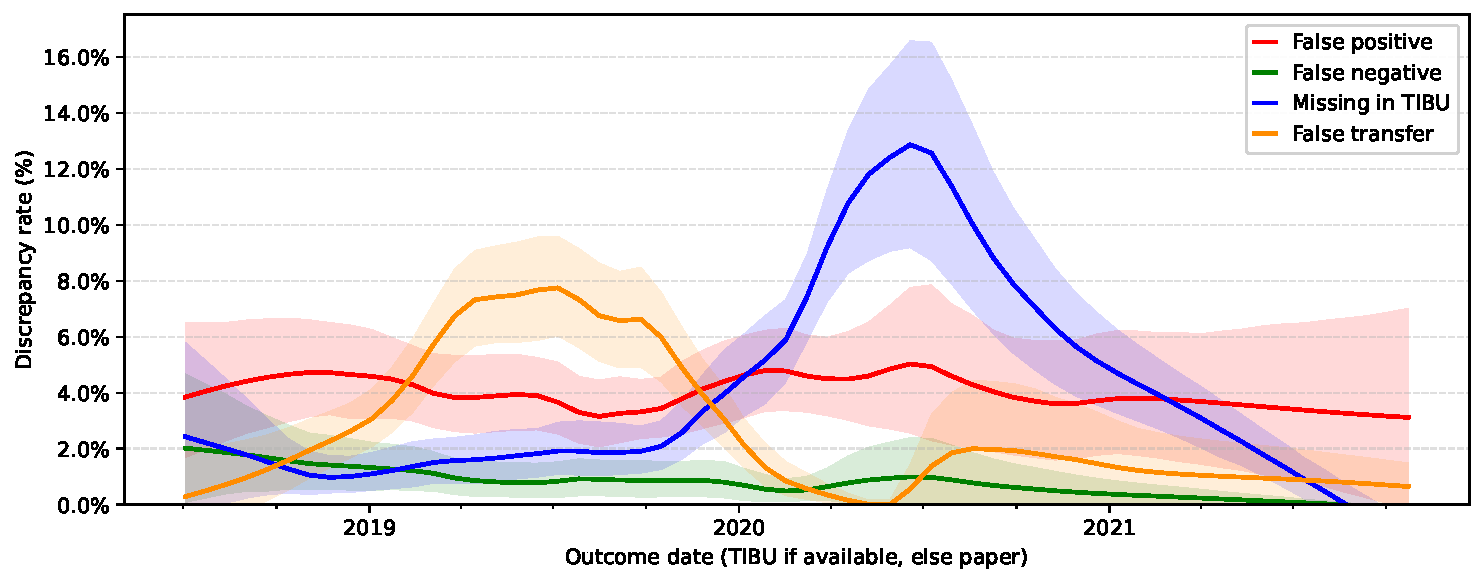
\includegraphics[width=0.85\textwidth]{fig_error_over_time.pdf}
    \caption{DQA error rates over time by outcome date (TIBU when available, paper otherwise). Lowess smooth with percentile bootstrap 95\% CI bands.}
    \label{fig:over_time}
\end{figure}

\noindent The dominant feature of the figure is a pronounced peak in the missing-in-TIBU rate (to roughly 15\%) for records with outcome dates in 2020 Q1--Q2, coinciding with the onset of the COVID-19 pandemic response in Kenya. Of the 116 missing-in-TIBU records in the classifiable sample, 63 fall in these two quarters. \texttt{NC} is a TIBU interim code denoting that treatment is still in progress; treating it as equivalent to blank (rather than as a medical failure) rolls the affected records into the missing-in-TIBU category, which accounts for 76 of the 116 (the remaining 40 have TIBU entirely blank). False-positive and false-negative rates are low and roughly flat across the study period.

A sensitivity check using paper-registry outcome dates throughout (rather than TIBU date with paper fallback for missing-in-TIBU records) is reported in Appendix~\ref{sec:appendix_paper_dates}. The COVID-era spike in missing-in-TIBU remains clearly visible there, confirming that it is driven by when outcomes actually occurred (as captured on paper), not by when TIBU happened to record them.

\subsection{Where did errors occur?}
\label{sec:errors_where}

Table~\ref{tbl:clinic_errors} reports false-positive, false-negative, and missing-in-TIBU rates stratified by province, urbanicity, and clinic size. In the full sample (left panel), error rates appear elevated at small clinics, in two provinces (Eastern South and Rift Valley South), and in rural areas. However, this concentration traces almost entirely to two specific clinics (IDs 0 and 115), whose missing-in-TIBU rates of $12.7\%$ and $15.4\%$ are an order of magnitude above the study-wide rate of $3.8\%$. These two clinics are responsible for the COVID-era reporting gap visible in Figure~\ref{fig:over_time}: 50 of the 116 missing-in-TIBU records in the sample come from them, inidcating that at these clinics paper-registry entries continued through the pandemic but TIBU outcomes were largely not recorded. 

The right panel of Table~\ref{tbl:clinic_errors} repeats the breakdown after excluding these clinics 0 and 115, to allow for a comparison of error rates with and without the COVID-era reporting gap.  Once those two clinics are removed, the missing-in-TIBU rate falls from $3.8\%$ to $2.4\%$, and the within-stratum rates flatten: the small-clinic missing rate drops from $5.1\%$ to $2.8\%$, the rural rate from $3.3\%$ to $0.9\%$, and the Eastern-South and Rift-Valley-South rates from $8.7\%$ and $7.7\%$ to $0.8\%$ and $0.0\%$ respectively. False-positive and false-negative rates barely move under the exclusion, consistent with their being dispersed across the country rather than concentrated. 

A multivariate logistic regression with patient, clinic, and record-age covariates corroborates this picture (Appendix~\ref{sec:appendix_logit}): once the two clinics are excluded, the only systematic predictor of missing-in-TIBU is record age, and there is no evidence of patient- or clinic-level structural predictors.

\begin{table}[H]
    \centering
    \caption{DQA error rates by province, urbanicity, and clinic size; full sample (left panel) and excluding the two clinics responsible for the COVID-era missing-in-TIBU spike (right panel).}
    \label{tbl:clinic_errors}
    \resizebox{\textwidth}{!}{\newsavebox{\ClinicErrBox}
\savebox{\ClinicErrBox}{\footnotesize{
\begin{tabular}{l|rr|rr|rr|rr|rr}
\hline\hline \\[-8pt]
& \multicolumn{2}{c|}{} & \multicolumn{2}{c|}{False positive} & \multicolumn{2}{c|}{False negative} & \multicolumn{2}{c|}{Missing in TIBU} & \multicolumn{2}{c}{False transfer} \\
& $N$ & (\%) & $N$ & (\%) & $N$ & (\%) & $N$ & (\%) & $N$ & (\%) \\
\hline \\[-8pt]
\textit{By province} &  &  &  &  &  &  &  &  &  & \\
\quad Central & 27 & (0.8\%) & 0 & (0.0\%) & 0 & (0.0\%) & 13 & (48.1\%) & 0 & (0.0\%) \\
\quad Coast & 708 & (21.4\%) & 18 & (2.5\%) & 4 & (0.6\%) & 13 & (1.8\%) & 6 & (0.8\%) \\
\quad Eastern North & 2 & (0.1\%) & 0 & (0.0\%) & 0 & (0.0\%) & 0 & (0.0\%) & 0 & (0.0\%) \\
\quad Eastern South & 264 & (8.0\%) & 8 & (3.0\%) & 2 & (0.8\%) & 24 & (9.1\%) & 12 & (4.5\%) \\
\quad Nairobi & 535 & (16.2\%) & 18 & (3.4\%) & 7 & (1.3\%) & 4 & (0.7\%) & 89 & (16.6\%) \\
\quad North Eastern & 821 & (24.8\%) & 66 & (8.0\%) & 6 & (0.7\%) & 2 & (0.2\%) & 19 & (2.3\%) \\
\quad Nyanza North & 392 & (11.9\%) & 6 & (1.5\%) & 7 & (1.8\%) & 3 & (0.8\%) & 2 & (0.5\%) \\
\quad Nyanza South & 40 & (1.2\%) & 1 & (2.5\%) & 0 & (0.0\%) & 0 & (0.0\%) & 0 & (0.0\%) \\
\quad Rift Valley North & 44 & (1.3\%) & 0 & (0.0\%) & 0 & (0.0\%) & 0 & (0.0\%) & 0 & (0.0\%) \\
\quad Rift Valley South & 425 & (12.9\%) & 15 & (3.5\%) & 3 & (0.7\%) & 37 & (8.7\%) & 4 & (0.9\%) \\
\quad Western & 31 & (0.9\%) & 2 & (6.5\%) & 1 & (3.2\%) & 1 & (3.2\%) & 0 & (0.0\%) \\
\rule{0pt}{14pt}\textit{By urban/rural} &  &  &  &  &  &  &  &  &  & \\
\quad Urban & 1,118 & (33.8\%) & 30 & (2.7\%) & 10 & (0.9\%) & 21 & (1.9\%) & 95 & (8.5\%) \\
\quad Rural & 2,167 & (65.5\%) & 104 & (4.8\%) & 20 & (0.9\%) & 76 & (3.5\%) & 37 & (1.7\%) \\
\rule{0pt}{14pt}\textit{By clinic size} &  &  &  &  &  &  &  &  &  & \\
\quad Large clinic & 1,273 & (38.5\%) & 39 & (3.1\%) & 10 & (0.8\%) & 24 & (1.9\%) & 90 & (7.1\%) \\
\quad Small clinic & 2,033 & (61.5\%) & 95 & (4.7\%) & 20 & (1.0\%) & 90 & (4.4\%) & 42 & (2.1\%) \\
\rule{0pt}{14pt}All & 3,306 & (100.0\%) & 134 & (4.1\%) & 30 & (0.9\%) & 114 & (3.4\%) & 132 & (4.0\%) \\
\hline\hline
\end{tabular}}}
\begin{minipage}{\wd\ClinicErrBox}
\usebox{\ClinicErrBox}
\par\vspace{4pt}\noindent
\footnotesize{\textit{Note:} Urban/rural classification is based on clinic records. Large clinics are those with at least 7 patients registered in TIBU (median); small clinics are those with fewer.}
\end{minipage}}
\end{table}

\subsection{Who experienced errors?}
\label{sec:errors_who}

Table~\ref{tbl:patient_errors} reports the same error rates broken down by individual patient and disease characteristics, again with a side-by-side panel excluding the two COVID-impacted clinics. Errors and significant correlations present in the left panel attenuate sharply in the right: the missing-in-TIBU rate among males falls from $3.6\%$ to $1.2\%$, the rate among the 15--34 age band falls from $2.6\%$ to $0.9\%$, the HIV-positive rate from $3.0\%$ to $1.6\%$, and so on across all rows. False-positive and false-negative rates are largely unchanged. As with the clinic-level breakdown, the multivariate model in Appendix~\ref{sec:appendix_logit} confirms that no patient characteristic independently predicts missingness once the two clinics are excluded; the apparent demographic gradients in the left panel are picking up the demographic profile of those two clinics rather than any general pattern.

\begin{table}[H]
    \centering
    \caption{DQA error rates by individual and disease characteristics; full sample (left panel) and excluding the two COVID-impacted clinics (right panel).}
    \label{tbl:patient_errors}
    \resizebox{\textwidth}{!}{\newsavebox{\PatientErrBox}
\savebox{\PatientErrBox}{\footnotesize{
\begin{tabular}{l|rr|rr|rr|rr||rr|rr|rr|rr}
\hline\hline \\[-8pt]
& \multicolumn{8}{c||}{\textbf{All clinics}} & \multicolumn{8}{c}{\textbf{Excluding clinics 0 and 115}} \\
\cline{2-9}\cline{10-17} \\[-8pt]
& \multicolumn{2}{c|}{} & \multicolumn{2}{c|}{False positive} & \multicolumn{2}{c|}{False negative} & \multicolumn{2}{c||}{Missing in TIBU} & \multicolumn{2}{c|}{} & \multicolumn{2}{c|}{False positive} & \multicolumn{2}{c|}{False negative} & \multicolumn{2}{c}{Missing in TIBU} \\
& $N$ & (\%) & $N$ & (\%) & $N$ & (\%) & $N$ & (\%) & $N$ & (\%) & $N$ & (\%) & $N$ & (\%) & $N$ & (\%) \\
\hline \\[-8pt]
\textit{Individual characteristics} &  &  &  &  &  &  &  &  &  &  &  &  &  &  &  & \\
\quad Male & 1,872 & (63.4\%) & 19 & (1.0\%) & 14 & (0.7\%) & 68 & (3.6\%) & 1,637 & (63.0\%) & 18 & (1.1\%) & 14 & (0.9\%) & 20 & (1.2\%) \\
\rule{0pt}{14pt}\textit{Age group} &  &  &  &  &  &  &  &  &  &  &  &  &  &  &  & \\
\quad $<$15 & 420 & (14.2\%) & 1 & (0.2\%) & 3 & (0.7\%) & 5 & (1.2\%) & 366 & (14.1\%) & 1 & (0.3\%) & 3 & (0.8\%) & 3 & (0.8\%) \\
\quad 15--34 & 1,334 & (45.2\%) & 18 & (1.3\%) & 11 & (0.8\%) & 35 & (2.6\%) & 1,170 & (45.0\%) & 17 & (1.5\%) & 11 & (0.9\%) & 11 & (0.9\%) \\
\quad 35--54 & 866 & (29.3\%) & 6 & (0.7\%) & 5 & (0.6\%) & 29 & (3.3\%) & 755 & (29.0\%) & 6 & (0.8\%) & 5 & (0.7\%) & 11 & (1.5\%) \\
\quad 55+ & 297 & (10.1\%) & 6 & (2.0\%) & 2 & (0.7\%) & 8 & (2.7\%) & 273 & (10.5\%) & 6 & (2.2\%) & 2 & (0.7\%) & 3 & (1.1\%) \\
\rule{0pt}{14pt}\textit{Disease characteristics} &  &  &  &  &  &  &  &  &  &  &  &  &  &  &  & \\
\quad Bacteriologically confirmed & 2,041 & (69.1\%) & 25 & (1.2\%) & 14 & (0.7\%) & 61 & (3.0\%) & 1,788 & (68.8\%) & 24 & (1.3\%) & 14 & (0.8\%) & 24 & (1.3\%) \\
\quad Extrapulmonary & 331 & (11.2\%) & 2 & (0.6\%) & 0 & (0.0\%) & 8 & (2.4\%) & 302 & (11.6\%) & 2 & (0.7\%) & 0 & (0.0\%) & 5 & (1.7\%) \\
\quad Retreatment & 275 & (9.3\%) & 5 & (1.8\%) & 1 & (0.4\%) & 5 & (1.8\%) & 250 & (9.6\%) & 5 & (2.0\%) & 1 & (0.4\%) & 2 & (0.8\%) \\
\quad HIV positive & 667 & (22.6\%) & 6 & (0.9\%) & 8 & (1.2\%) & 20 & (3.0\%) & 577 & (22.2\%) & 5 & (0.9\%) & 8 & (1.4\%) & 9 & (1.6\%) \\
\rule{0pt}{14pt}All & 2,953 & (100.0\%) & 31 & (1.0\%) & 21 & (0.7\%) & 112 & (3.8\%) & 2,599 & (100.0\%) & 30 & (1.2\%) & 21 & (0.8\%) & 62 & (2.4\%) \\
\hline\hline
\end{tabular}}}
\begin{minipage}{\wd\PatientErrBox}
\usebox{\PatientErrBox}
\par\vspace{4pt}\noindent
\footnotesize{\textit{Note:} Each row shows the count and rate of records matching the row label, and the count and rate of each error type within those records. Rows are not mutually exclusive (e.g.\ a male HIV-positive patient appears in both rows). The right panel excludes clinic IDs 0 and 115 (the two clinics responsible for the COVID-era missing-in-TIBU spike).}
\end{minipage}}
\end{table}

\iffalse  % --- §4.4 Record Age and Reporting Lag commented out (Apr 2026) ---
\subsection{Record Age and Reporting Lag by Error Type}
\label{sec:lag}

Table~\ref{tbl:lag} reports two measures of record age at the TIBU extract snapshot, stratified by error type: (i) \textbf{record age}, measured from patient registration to the snapshot, and (ii) \textbf{reporting lag}, measured from the TIBU outcome date to the snapshot. The expected pattern under normal TIBU operation is a reporting lag of roughly 6--9 months after a drug-sensitive outcome date (to allow for paper-register close-out and clerical transcription); systematic deviations in the lag distribution across error categories can indicate particular failure modes.

\begin{table}[H]
    \centering
    \caption{Record age and reporting lag (days) at the TIBU snapshot, by error category.}
    \label{tbl:lag}
    \newsavebox{\CorrLagBox}
\savebox{\CorrLagBox}{\scriptsize{
\begin{tabular}{l|rr|rrr|rrr}
\hline\hline \\[-8pt]
 & & & \multicolumn{3}{c|}{Record age (days)}   & \multicolumn{3}{c}{Reporting lag (days)} \\
Error type & $N$ & (\%) & $n$ & Mean & Median & $n$ & Mean & Median \\
\hline \\[-8pt]
\textcolor{red}{False positive (Type I)} & 31 & (1.0\%) & 31 & 1020 & 982 & 31 & 873 & 807 \\
\textcolor{green!60!black}{False negative (Type II)} & 21 & (0.7\%) & 21 & 1033 & 1019 & 21 & 964 & 1005 \\
\textcolor{blue}{Missing in TIBU} & 112 & (3.8\%) & 112 & 920 & 844 & 110 & 749 & 690 \\
No error & 2,789 & (94.4\%) & 2,789 & 1029 & 1002 & 2,789 & 847 & 848 \\
\hline\hline
\end{tabular}}}
\begin{minipage}{\wd\CorrLagBox}
\usebox{\CorrLagBox}
\par\vspace{4pt}\noindent
\scriptsize{\textit{Note:} The TIBU snapshot is taken to be 1 January 2022, based on the latest treatment-outcome dates in the extract clustering in late December 2021. Record age is measured from registration to snapshot; reporting lag is measured from TIBU outcome date to snapshot. Column $n$ gives the number of records with a valid date; $N$ counts all records in the error category.}
\end{minipage}
\end{table}

\noindent False-negative records have a notably longer reporting lag than no-error records (median $1{,}026$ vs.\ $850$ days) but a nearly identical record age (median $1{,}040$ vs.\ $1{,}004$ days). The asymmetry is informative. Reporting lag is measured from the \emph{TIBU} outcome date, which for a false-negative record is the early failure determination TIBU made (e.g., LTFU declared at month~6) rather than the later completion the patient actually reached: median TIBU outcome dates for false-negative records are roughly five months earlier than for no-error records, while median \emph{paper} outcome dates are only two months earlier. Record age, which depends only on registration date, shows no such gap---registration dates for both categories are drawn from the same April 2018--December 2019 window.

\noindent Stratifying instead by paper outcome date (the ground-truth timestamp) shows a false-negative rate that is roughly flat across the study period (0.4--1.5\% per quarter from 2018 Q3 through 2020 Q2), and the 22 false-negative records are spread across 12 clinics with no overlap with the two clinics responsible for the COVID-era missing-in-TIBU spike. On this reading, the apparent concentration of false negatives at long reporting lags is largely an artifact of where TIBU's (incorrect) outcome date lands on the calendar---an early ``failed'' closure is mechanically older than a later ``completed'' closure would have been---rather than evidence of a temporal gradient in the underlying error rate.
\fi  % --- end commented-out §4.4 ---

\iffalse  % --- §4.6 Supplementary record-age views commented out (Apr 2026) ---
\subsection{Supplementary views: error rates against record-age axes}

Figures~\ref{fig:age_reg}--\ref{fig:density} present the same underlying data as Figure~\ref{fig:over_time} against record-age axes rather than calendar time; they are included as supplementary confirmation that the COVID-era missing-in-TIBU peak is not an artifact of the time axis. Figure~\ref{fig:age_reg} plots error rates against record age at snapshot (days from registration to 1 January 2022); Figure~\ref{fig:age_out} plots them against reporting lag (days from outcome date to snapshot, with the axis inverted so that calendar time reads left-to-right like Figure~\ref{fig:over_time}); Figure~\ref{fig:density} compares the empirical distributions of reporting lag across error categories. The COVID-era missing-in-TIBU peak is visible as a left-edge spike in Figure~\ref{fig:age_reg} (records registered in late 2019, whose treatments completed in 2020) and as a mid-2020 spike in Figure~\ref{fig:age_out}; Figure~\ref{fig:density} shows the missing-in-TIBU distribution shifted noticeably toward shorter reporting lags, which is the same COVID-era concentration viewed as a cumulative distribution.

\begin{figure}[H]
    \centering
    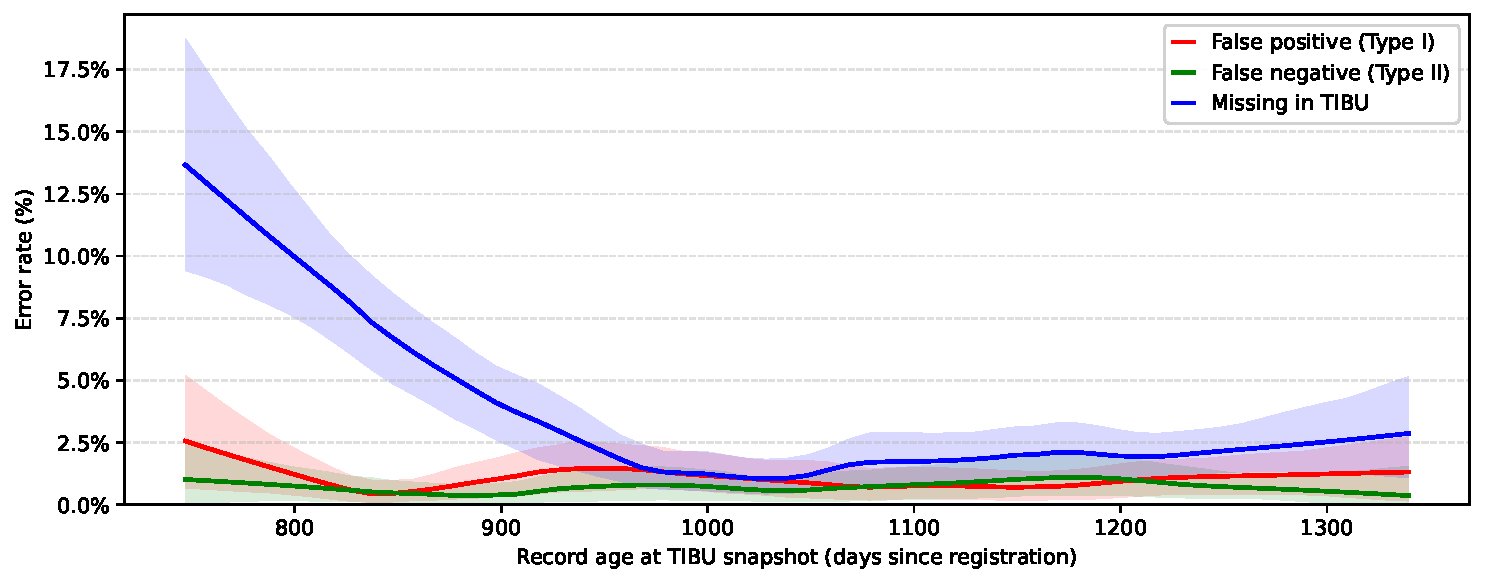
\includegraphics[width=0.85\textwidth]{fig_error_by_age_reg.pdf}
    \caption{DQA error rates by record age at TIBU snapshot (days since registration). Lowess smooth with percentile bootstrap 95\% CI bands.}
    \label{fig:age_reg}
\end{figure}

\begin{figure}[H]
    \centering
    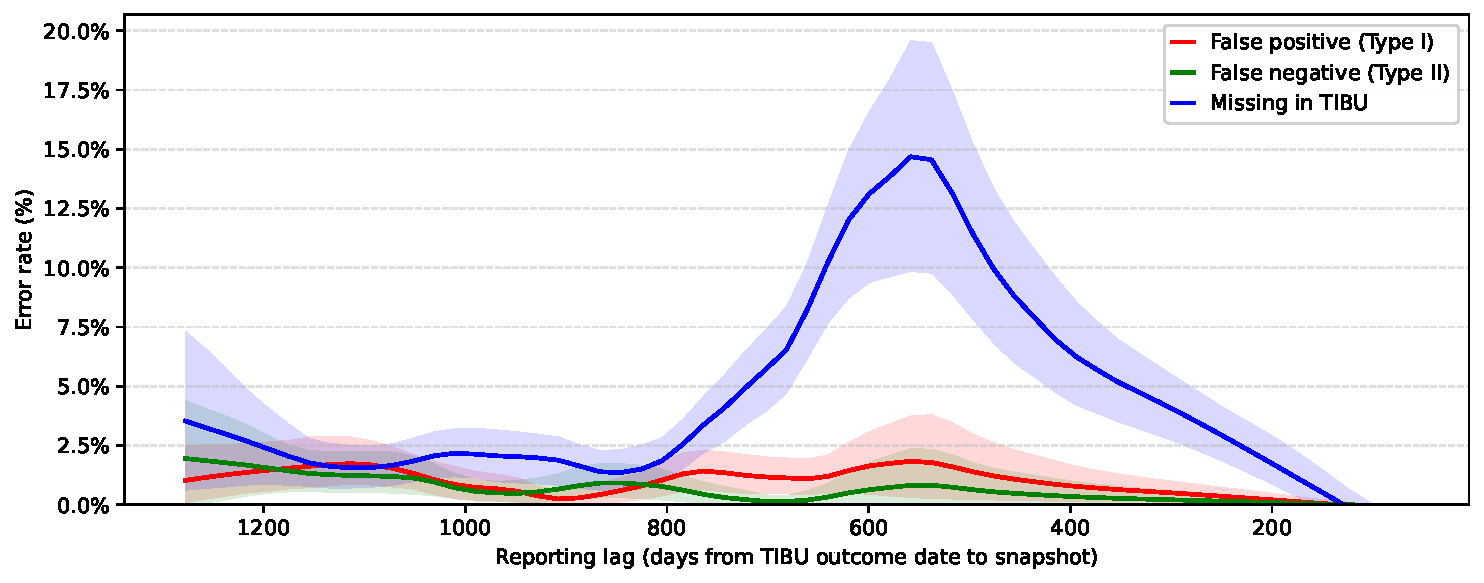
\includegraphics[width=0.85\textwidth]{fig_error_by_age_out.pdf}
    \caption{DQA error rates by reporting lag (days from the outcome date to the TIBU snapshot); x-axis inverted so older outcomes are on the left and recent outcomes on the right. Lowess smooth with percentile bootstrap 95\% CI bands. For missing-in-TIBU records (TIBU blank) the paper-registry outcome date is used in place of the TIBU outcome date.}
    \label{fig:age_out}
\end{figure}

\begin{figure}[H]
    \centering
    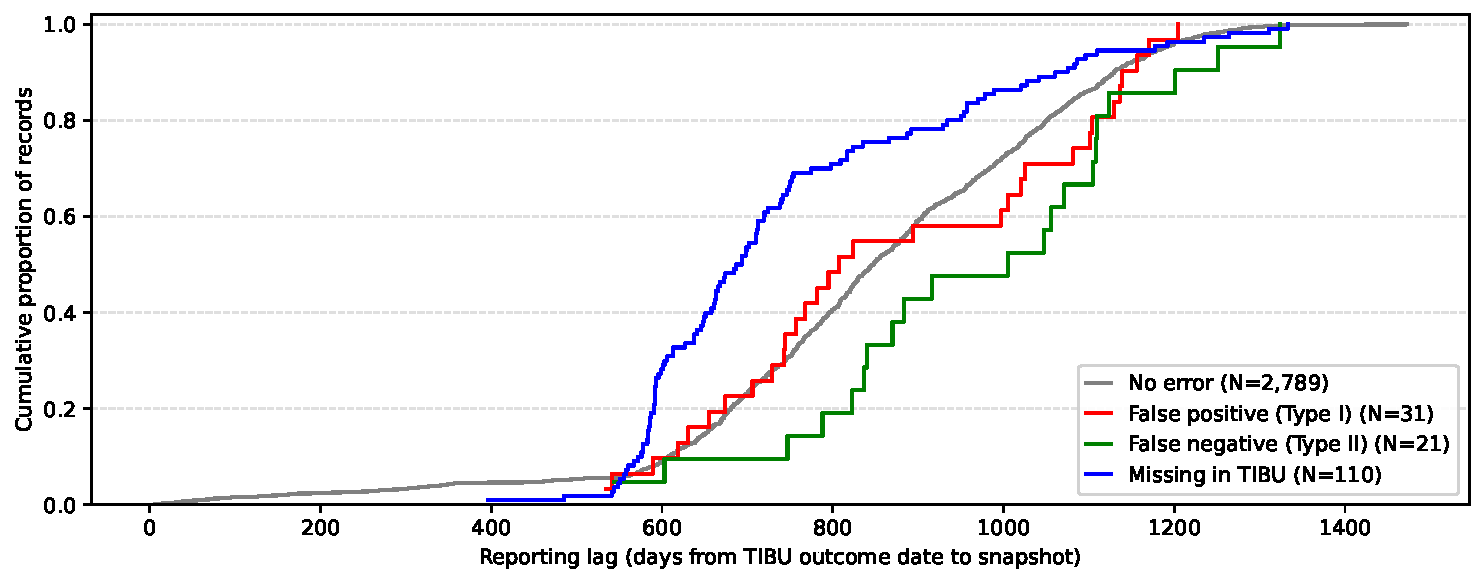
\includegraphics[width=0.85\textwidth]{fig_error_density.pdf}
    \caption{Empirical cumulative distribution function (ECDF) of reporting lag, by error category; the curve at each $x$ gives the fraction of records in that category with reporting lag $\leq x$. Separation from the no-error curve indicates where on the age axis each error type concentrates.}
    \label{fig:density}
\end{figure}
\fi  % --- end commented-out §4.6 ---

% =============================================================================
\section{Incorporating Date Fields to Assess Outcome Errors}
\label{sec:date_errors}
% =============================================================================

Up to this point we have treated the paper register as ground truth. But the audit itself can err: through transcription mistakes, by matching a paper record to the wrong patient, or by transcribing an out-of-date entry for the right patient. The outcome-date comparison in this section speaks directly to the last of these failure modes.

Although an audit of the date fields was not a priority of the trial's data-quality programme, the audit team transcribed dates alongside outcomes for $3{,}186$ of the $3{,}645$ audit records ($87.4\%$). A comparison of outcome dates from TIBU and the paper audit can provide insight on the nature of the inconsistency between TIBU and the paper records as digitized in the audit.

For DQA-matched records where both the TIBU and paper outcome dates are parseable, we can compare the two directly (Table~\ref{tbl:date_agree} and Figure~\ref{fig:tibu_vs_paper_date}).

\begin{table}[H]
    \centering
    \caption{TIBU--paper outcome-date agreement, by outcome-error category.}
    \label{tbl:date_agree}
    \newsavebox{\DateAgreeBox}
\savebox{\DateAgreeBox}{\scriptsize{
\begin{tabular}{l|r|rrrrr|rr}
\hline\hline \\[-8pt]
 & & \multicolumn{5}{c|}{$|$TIBU $-$ paper$|$ (days)} & \multicolumn{2}{c}{TIBU date is} \\
Category & $N$ & $\leq$ 7 days & 8--30 days & 31--90 days & 91--180 days & $>$180 days & Earlier & Later \\
\hline \\[-8pt]
\textcolor{black}{Concordant} & 2,766 & 2140 (77.4\%) & 203 (7.3\%) & 136 (4.9\%) & 51 (1.8\%) & 236 (8.5\%) & 371 (13.4\%) & 450 (16.3\%) \\
\textcolor{red}{False positive} & 57 & 9 (15.8\%) & 4 (7.0\%) & 6 (10.5\%) & 24 (42.1\%) & 14 (24.6\%) & 6 (10.5\%) & 43 (75.4\%) \\
\textcolor{green!60!black}{False negative} & 21 & 2 (9.5\%) & 3 (14.3\%) & 5 (23.8\%) & 7 (33.3\%) & 4 (19.0\%) & 14 (66.7\%) & 6 (28.6\%) \\
\textcolor{orange!85!black}{False transfer} & 130 & 8 (6.2\%) & 7 (5.4\%) & 6 (4.6\%) & 50 (38.5\%) & 59 (45.4\%) & 117 (90.0\%) & 6 (4.6\%) \\
\hline\hline
\end{tabular}}}
\begin{minipage}{\wd\DateAgreeBox}
\usebox{\DateAgreeBox}
\par\vspace{4pt}\noindent
\scriptsize{\textit{Note:} Denominator is records where both the TIBU and paper outcome dates are non-blank and parseable. Missing-in-TIBU records cannot appear (TIBU date is blank by construction); their temporal pattern is in Figure~\ref{fig:over_time}. ``TIBU earlier'' and ``TIBU later'' together sum to $<$ 100\% because some records agree exactly.}
\end{minipage}
\end{table}

\begin{figure}[H]
    \centering
    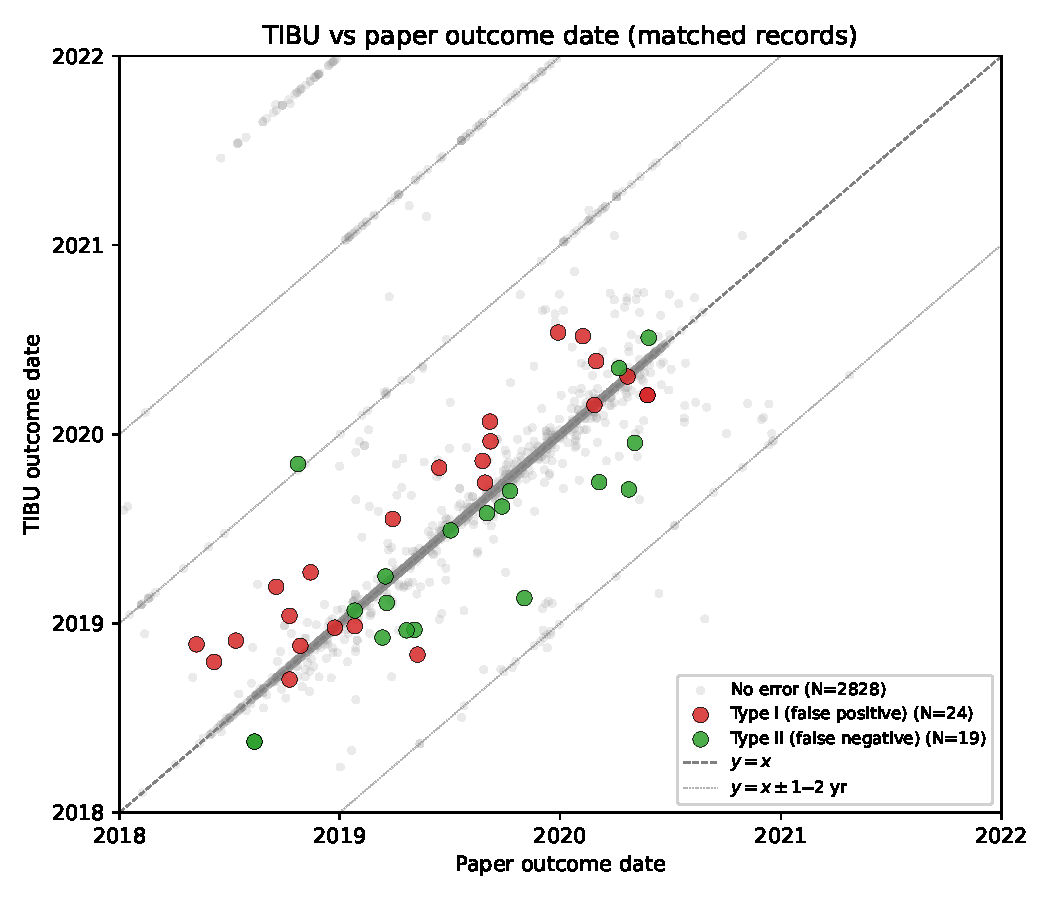
\includegraphics[width=0.78\textwidth]{fig_tibu_vs_paper_date.pdf}
    \caption{TIBU outcome date vs.\ paper outcome date for DQA-matched records with parseable dates on both sides (axes clipped to the 2018--2022 study window). Points on the $y=x$ dashed line agree exactly. False-positive points (red) sit predominantly above the line (TIBU later), false-negative points (green) predominantly below (TIBU earlier). The multiple parallel 45-degree lines arise because it is common for TIBU and the paper audit to disagree on the year of the record (without changing the recorded outcome).}
    \label{fig:tibu_vs_paper_date}
\end{figure}

Among no-error records the two dates agree to within a week $\sim 78\%$ of the time, with a small symmetric tail. The pattern is qualitatively different for the two error classes: for false-positive records, TIBU is \emph{later} than the audit-transcribed paper date in $16$ of $23$ cases ($\sim 70\%$); for false-negative records, TIBU is \emph{earlier} in $13$ of $18$ ($\sim 72\%$). This suggests that the majority of apparent false positives are not in fact errors, but result from the paper audit occasionally having employed less up-to-date records than TIBU.

Operationalizing this reading, we define a \emph{date-gated} sensitivity classification: a TIBU--paper outcome disagreement is counted as an error only when the paper outcome date is strictly later than the TIBU outcome date. When TIBU is the more recent reading, the record is treated as concordant on the assumption that TIBU reflects a post-audit paper update. Missing-in-TIBU is unchanged because TIBU is blank by construction. Table~\ref{tbl:sensitivity} shows the resulting headline-vs-gated comparison; under the gate, the false-positive rate falls by roughly half (from $1.05\%$ to $0.51\%$), the false-negative rate falls only slightly (from $0.71\%$ to $0.58\%$), and the missing-in-TIBU rate is unchanged ($3.79\%$). Equivalent breakdowns of Tables~\ref{tbl:clinic_errors} and~\ref{tbl:patient_errors} and Figure~\ref{fig:over_time} under the date-gated definition are collected in Appendix~\ref{sec:appendix_gated}.

\begin{table}[H]
    \centering
    \caption{Headline vs.\ date-gated DQA error counts and rates.}
    \label{tbl:sensitivity}
    \newsavebox{\SensBox}
\savebox{\SensBox}{\scriptsize{
\begin{tabular}{l|rr|rr}
\hline\hline \\[-8pt]
 & \multicolumn{2}{c|}{Headline} & \multicolumn{2}{c}{Date-gated} \\
Discrepancy type & $N$ & Rate & $N$ & Rate \\
\hline \\[-8pt]
\textcolor{red}{False positive} & 134 & 4.05\% & 91 & 2.75\% \\
\textcolor{green!60!black}{False negative} & 30 & 0.91\% & 24 & 0.73\% \\
\textcolor{orange!85!black}{False transfer} & 132 & 3.99\% & 126 & 3.81\% \\
\textcolor{blue}{Missing in TIBU} & 114 & 3.45\% & 114 & 3.45\% \\
\hline\hline
\end{tabular}}}
\begin{minipage}{\wd\SensBox}
\usebox{\SensBox}
\par\vspace{4pt}\noindent
\scriptsize{\textit{Note:} Denominator is the $N = 3,306$ classifiable matched records. Under the date-gated definition, a TIBU--paper outcome disagreement is counted as an error only when the paper outcome date is strictly later than the TIBU outcome date; otherwise the record is treated as concordant on the assumption that TIBU reflects a post-audit paper update. The rule cannot be applied to records with an unparseable date on either side ($n = 77$ false-positive and $n = 9$ false-negative records), and such records preserve their headline classification. Missing-in-TIBU is unaffected since TIBU is blank by construction.}
\end{minipage}
\end{table}

%%%% Everything after this comment is preserved but commented out.
\iffalse



 but did not treat them as a priority. The paper-date column in the audit therefore cannot be treated as ground truth for date accuracy in the way that paper outcomes can. We consequently keep this section narrow, focused on what the date comparison reveals about the outcome-error counts in \S\ref{sec:outcome_errors} -- in particular, that many of the apparent false-positive records are not TIBU errors at all.

\noindent \textbf{Caveat on the paper figures.} The audit team's primary focus was the treatment-outcome field; dates were transcribed alongside outcomes but were not a priority for careful entry. The paper-date issues in Table~\ref{tbl:date_quality} may therefore reflect the audit's transcription quality on the date column, not the underlying paper register.

\subsection{Date completeness}

Within TIBU, the registration, treatment-start, and outcome dates are each blank in $5$--$9\%$ of records (Table~\ref{tbl:date_quality}); the TIBU outcome date is the most often blank, the same failure mode driving the missing-in-TIBU rate in \S\ref{sec:outcome_errors}. The paper outcome-date column is more uneven, but per the caveat above, that figure reflects the audit transcription rather than the underlying register.

\begin{table}[H]
    \centering
    \caption{Completeness and plausibility of date fields, by source.}
    \label{tbl:date_quality}
    \newsavebox{\DateQualityBox}
\savebox{\DateQualityBox}{\scriptsize{
\begin{tabular}{lrrrrr}
\hline\hline \\[-8pt]
Field & $N$ & Blank & Unparseable & Out of range & Valid \\
\hline \\[-8pt]
\textit{Paper registry} (audit records) & & & & & \\
\quad Paper outcome date & 3,645 & 459 (12.6\%) & 30 (0.8\%) & 5 (0.1\%) & 3,151 (86.4\%) \\
\rule{0pt}{10pt}\textit{TIBU} (study-clinic extract) & & & & & \\
\quad TIBU clinical registration date & 17,740 & 978 (5.5\%) & 4 (0.0\%) & 0 (0.0\%) & 16,758 (94.5\%) \\
\quad TIBU treatment-start date & 17,740 & 1,001 (5.6\%) & 0 (0.0\%) & 0 (0.0\%) & 16,739 (94.4\%) \\
\quad TIBU outcome date & 17,740 & 1,608 (9.1\%) & 0 (0.0\%) & 1 (0.0\%) & 16,131 (90.9\%) \\
\hline\hline
\end{tabular}}}
\begin{minipage}{\wd\DateQualityBox}
\usebox{\DateQualityBox}
\par\vspace{4pt}\noindent
\scriptsize{\textit{Note:} Plausible range = 2017-01-01 through 2022-06-30. ``Unparseable'' values are nonblank strings that could not be parsed as a date; ``out of range'' are parseable dates outside the plausible window.}
\end{minipage}
\end{table}

\iffalse  % --- §5.x Internal consistency + triangulation commented out (Apr 2026) ---
\subsection{Internal consistency within TIBU}

Given three TIBU date fields per record (clinical registration, treatment start, outcome), we can check whether they occur in the expected clinical order and whether the implied treatment duration is plausible. Table~\ref{tbl:date_consistency} reports violations. Roughly 6\% of records have an outcome date before the clinical registration date, 3\% have an outcome before treatment start, and 8\% imply a treatment duration under 30 days -- any of which would render the record's reporting-lag and age statistics unreliable.

An additional quirk not tabulated: the clinical registration date (\texttt{dateofregistration}) is on or after the treatment-start date (\texttt{dateoftreatmentstarted}) in about 90\% of records, with a typical gap of a week or two. We read this as a TIBU data-entry convention (case formally registered into TIBU shortly after treatment initiation) rather than a data-quality issue, and therefore do not count it as a violation in the table.

\begin{table}[H]
    \centering
    \caption{Internal consistency of TIBU date fields.}
    \label{tbl:date_consistency}
    \newsavebox{\DateConsistBox}
\savebox{\DateConsistBox}{\scriptsize{
\begin{tabular}{lrr}
\hline\hline \\[-8pt]
Invariant violation & Denominator & Violations \\
\hline \\[-8pt]
Treatment start after outcome date & 15,577 & 415 (2.7\%) \\
Clinical registration after outcome date & 15,578 & 913 (5.9\%) \\
Treatment duration $<$ 30 days & 15,577 & 1,243 (8.0\%) \\
Treatment duration $>$ 900 days & 15,577 & 0 (0.0\%) \\
\hline\hline
\end{tabular}}}
\begin{minipage}{\wd\DateConsistBox}
\usebox{\DateConsistBox}
\par\vspace{4pt}\noindent
\scriptsize{\textit{Note:} Denominator for each row is the number of study-clinic records (of $N=17,160$) with a valid (non-blank, in-range) date in both fields being compared. Violations count records where the ordering invariant fails.}
\end{minipage}
\end{table}

\noindent \textbf{Triaging inconsistent records using the audit.} For a TIBU record with an internal inconsistency, which date field is wrong? If the record happens to be in the DQA-audited subset, the paper outcome date gives a second independent reading that can resolve the ambiguity. Table~\ref{tbl:date_triangulation} applies this to the three most common violation types. A simple heuristic decides each case: we call the TIBU \emph{outcome date} suspect when the paper outcome date is plainly later than the TIBU registration or treatment-start date (so the outcome really happened later than TIBU implies), and we call the TIBU outcome \emph{plausible} when the paper outcome date is within 30 days of the TIBU outcome date (the outcome really did occur early and the TIBU field just contradicts the registration side). Across the three violation types, the paper audit resolves roughly half of the DQA-matched cases in a clear direction, which gives TIBU researchers a workable recipe for salvaging individual records: an internally inconsistent TIBU record with a paper audit counterpart can often be fixed with a single-column edit informed by the paper date.

\begin{table}[H]
    \centering
    \caption{Resolving TIBU internal-consistency violations via the paper audit date.}
    \label{tbl:date_triangulation}
    \newsavebox{\DateTriangleBox}
\savebox{\DateTriangleBox}{\scriptsize{
\begin{tabular}{lrrrr}
\hline\hline \\[-8pt]
 & & & \multicolumn{2}{c}{Paper audit date resolves violation} \\
Violation & Total & In audit & TIBU outcome suspect & TIBU outcome plausible \\
\hline \\[-8pt]
Outcome date before registration & 913 & 202 & 92 (46\%) & 52 (26\%) \\
Outcome date before treatment start & 415 & 78 & 13 (17\%) & 4 (5\%) \\
Treatment duration $<$ 30 days & 1,243 & 293 & 121 (41\%) & 172 (59\%) \\
\hline\hline
\end{tabular}}}
\begin{minipage}{\wd\DateTriangleBox}
\usebox{\DateTriangleBox}
\par\vspace{4pt}\noindent
\scriptsize{\textit{Note:} For each TIBU internal-consistency violation, ``In audit'' counts records in the DQA-matched subset (with a paper outcome date). The two rightmost columns apply a heuristic: we call the TIBU outcome \emph{suspect} when the paper date is consistent with the TIBU registration/treatment-start timeline (paper outcome clearly later), and \emph{plausible} when the paper date is within 30 days of the TIBU outcome date (confirming the outcome really did happen early). Neither column is mutually exclusive; some records are classified by both heuristics, or by neither.}
\end{minipage}
\end{table}
\fi  % --- end commented-out §5.x ---

\subsection{TIBU vs.\ paper outcome dates: many false positives are audit artifacts}

For DQA-matched records where both the TIBU and paper outcome dates are parseable, we can compare the two directly (Table~\ref{tbl:date_agree} and Figure~\ref{fig:tibu_vs_paper_date}). Among no-error records the two dates agree to within a week $\sim 78\%$ of the time, with a small symmetric tail. The pattern is qualitatively different for the two error classes: for false-positive records, TIBU is \emph{later} than the audit-transcribed paper date in $16$ of $24$ cases ($\sim 2/3$); for false-negative records, TIBU is \emph{earlier} in $14$ of $19$ ($\sim 3/4$).

\begin{table}[H]
    \centering
    \caption{TIBU--paper outcome-date agreement, by outcome-error category.}
    \label{tbl:date_agree}
    \newsavebox{\DateAgreeBox}
\savebox{\DateAgreeBox}{\scriptsize{
\begin{tabular}{l|r|rrrrr|rr}
\hline\hline \\[-8pt]
 & & \multicolumn{5}{c|}{$|$TIBU $-$ paper$|$ (days)} & \multicolumn{2}{c}{TIBU date is} \\
Category & $N$ & $\leq$ 7 days & 8--30 days & 31--90 days & 91--180 days & $>$180 days & Earlier & Later \\
\hline \\[-8pt]
\textcolor{black}{Concordant} & 2,766 & 2140 (77.4\%) & 203 (7.3\%) & 136 (4.9\%) & 51 (1.8\%) & 236 (8.5\%) & 371 (13.4\%) & 450 (16.3\%) \\
\textcolor{red}{False positive} & 57 & 9 (15.8\%) & 4 (7.0\%) & 6 (10.5\%) & 24 (42.1\%) & 14 (24.6\%) & 6 (10.5\%) & 43 (75.4\%) \\
\textcolor{green!60!black}{False negative} & 21 & 2 (9.5\%) & 3 (14.3\%) & 5 (23.8\%) & 7 (33.3\%) & 4 (19.0\%) & 14 (66.7\%) & 6 (28.6\%) \\
\textcolor{orange!85!black}{False transfer} & 130 & 8 (6.2\%) & 7 (5.4\%) & 6 (4.6\%) & 50 (38.5\%) & 59 (45.4\%) & 117 (90.0\%) & 6 (4.6\%) \\
\hline\hline
\end{tabular}}}
\begin{minipage}{\wd\DateAgreeBox}
\usebox{\DateAgreeBox}
\par\vspace{4pt}\noindent
\scriptsize{\textit{Note:} Denominator is records where both the TIBU and paper outcome dates are non-blank and parseable. Missing-in-TIBU records cannot appear (TIBU date is blank by construction); their temporal pattern is in Figure~\ref{fig:over_time}. ``TIBU earlier'' and ``TIBU later'' together sum to $<$ 100\% because some records agree exactly.}
\end{minipage}
\end{table}

\begin{figure}[H]
    \centering
    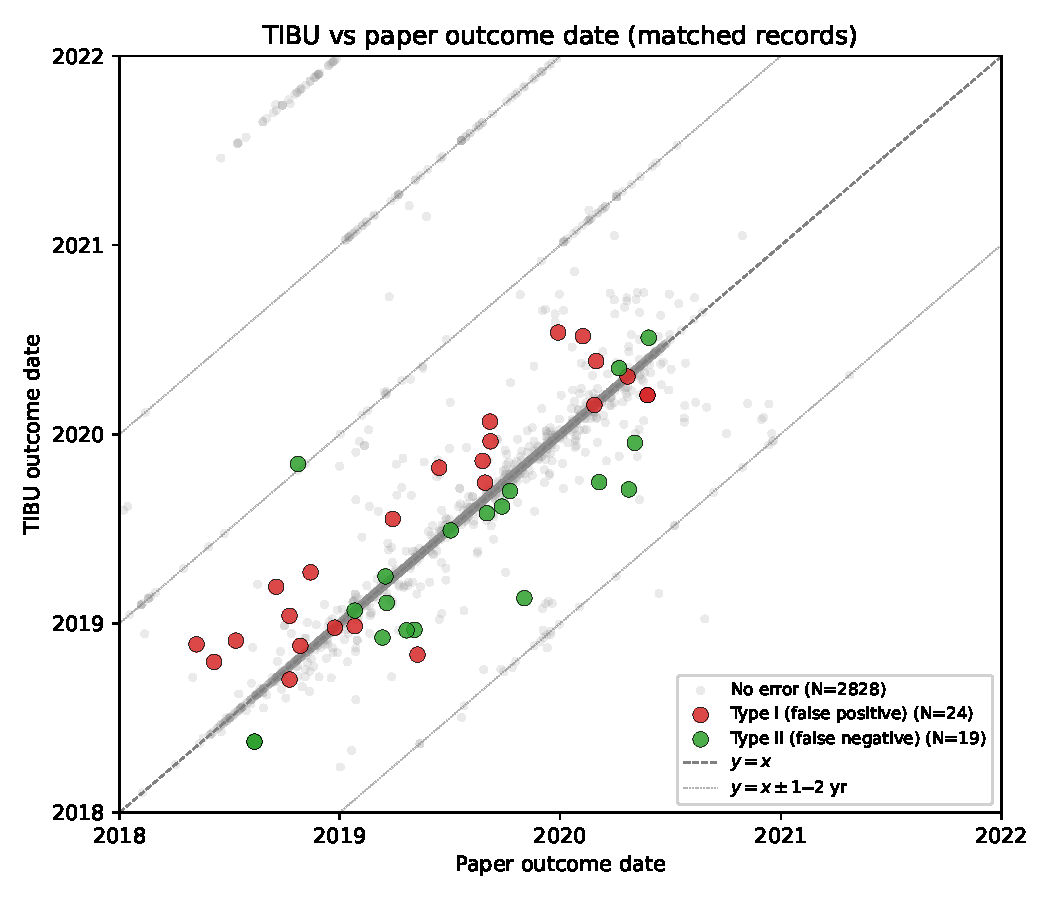
\includegraphics[width=0.75\textwidth]{fig_tibu_vs_paper_date.pdf}
    \caption{TIBU outcome date vs.\ paper outcome date for DQA-matched records with parseable dates on both sides (axes clipped to the 2018--2022 study window). Points on the $y=x$ dashed line agree exactly; the faint dotted lines mark $y = x \pm 1$ and $\pm 2$ years. False-positive points (red) sit predominantly above the $y=x$ line (TIBU later), false-negative points (green) predominantly below (TIBU earlier).}
    \label{fig:tibu_vs_paper_date}
\end{figure}

The false-positive pattern is the signature of an audit-snapshot artifact rather than a TIBU error. Each clinic's paper register continues to be updated as outcomes accrue; for a patient marked LTFU at month~3 on paper, then transcribed by the audit, who later returns and completes treatment, TIBU eventually reflects the completed outcome while the audit retains the earlier interim one. The TIBU outcome date in such a case lands \emph{after} the paper outcome date the audit captured -- exactly what we see in $\sim 2/3$ of false-positive records. The headline false-positive rate of $1.0\%$ in \S\ref{sec:outcome_errors} therefore likely overstates true TIBU misclassification; the residual is closer to $\sim 0.3\%$. By contrast, the false-negative and missing-in-TIBU rates are not affected by this caveat: paper at audit time clearly held a later outcome than TIBU's earlier closure (false negative), or paper had an outcome that TIBU never recorded at all (missing-in-TIBU). Both look like real TIBU lapses.

\iffalse  % --- Year-offset typos (date-only finding, not focused on outcome errors) ---
\noindent \textbf{Year-offset typos.} Figure~\ref{fig:tibu_vs_paper_date} reveals a second, distinct pattern: roughly $145$ matched records ($\sim 5\%$) fall on or near the $y = x + 365$d or $y = x + 730$d diagonals rather than on $y = x$. These are year-off typos -- same calendar day on both sides but a year (or two) apart. Almost all sit in the \emph{no-error} category ($145$ of $146$): a clerk mistyping the year does not change the recorded outcome, only the date attached to it. Year-offset typos do not drive outcome disagreements but would distort any analysis that uses TIBU or paper dates as axes if not censored.
\fi  % --- end commented-out year-offset paragraph ---
\fi  % --- end of section commented out per user marker (Apr 2026) ---

% =============================================================================
% --- Appendix divider page ---
\clearpage
\thispagestyle{empty}
\vspace*{\fill}
\begin{center}
{\Huge\bfseries Appendix}
\end{center}
\vspace*{\fill}
\clearpage

\appendix

% =============================================================================
\section{Sensitivity check: paper-registry outcome dates}
\label{sec:appendix_paper_dates}
% =============================================================================

Figure~\ref{fig:over_time_paper} replays the over-time analysis of \S\ref{sec:outcome_errors} using the paper-registry outcome date throughout, rather than TIBU's outcome date with paper fallback for missing-in-TIBU records. Records with no parseable paper date are excluded ($\sim 13\%$ of the classifiable sample). The COVID-era peak in missing-in-TIBU is unchanged in shape and magnitude, indicating that it is driven by when outcomes actually occurred (as captured on paper) and not by when TIBU happened to record them.

\begin{figure}[H]
    \centering
    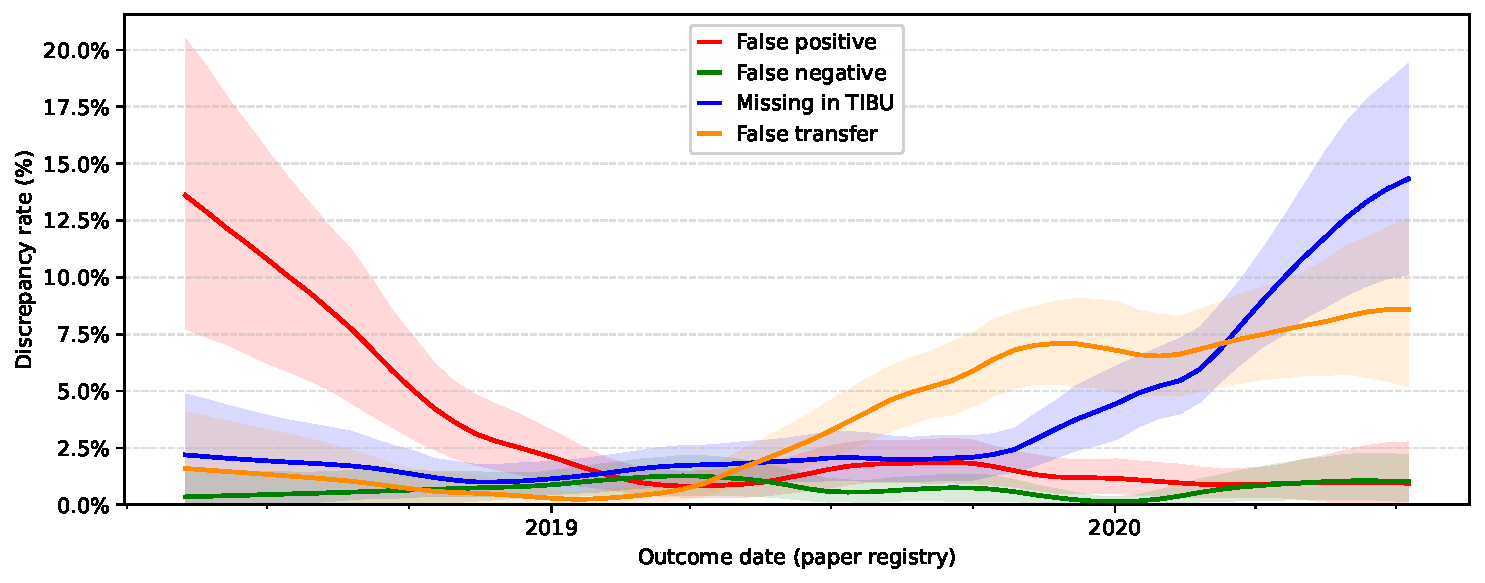
\includegraphics[width=0.85\textwidth]{fig_error_over_time_paper.pdf}
    \caption{DQA error rates over time using paper-registry outcome dates throughout. Records without a parseable paper date are excluded. Compare with Figure~\ref{fig:over_time}.}
    \label{fig:over_time_paper}
\end{figure}

% =============================================================================
\section{Error rates under the date-gated definition}
\label{sec:appendix_gated}
% =============================================================================

This appendix recreates the breakdowns of Tables~\ref{tbl:clinic_errors} and~\ref{tbl:patient_errors} and Figure~\ref{fig:over_time} under the date-gated classification introduced in \S\ref{sec:date_errors}. A matched record is counted as a TIBU error only if the TIBU and paper outcomes disagree \emph{and} the paper outcome date is strictly later than the TIBU outcome date; otherwise, on the reading that TIBU may reflect a post-audit paper update, the record is treated as concordant. Missing-in-TIBU is unchanged because TIBU is blank by construction. Records with an unparseable date on either side preserve their headline classification ($n = 8$ false-positive and $n = 3$ false-negative records). Headline-vs-gated marginal totals are in Table~\ref{tbl:sensitivity}. As in the body, each table presents two side-by-side panels: the full classifiable sample on the left, and the same breakdown excluding the two COVID-impacted clinics on the right.

\begin{table}[H]
    \centering
    \caption{DQA error rates by province, urbanicity, and clinic size, under the date-gated definition. Compare with Table~\ref{tbl:clinic_errors}.}
    \label{tbl:clinic_errors_gated}
    \resizebox{\textwidth}{!}{\newsavebox{\ClinicErrBoxGated}
\savebox{\ClinicErrBoxGated}{\scriptsize{
\begin{tabular}{l|rr|rr|rr|rr}
\hline\hline \\[-8pt]
& \multicolumn{2}{c|}{} & \multicolumn{2}{c|}{False positive} & \multicolumn{2}{c|}{False negative} & \multicolumn{2}{c}{Missing in TIBU} \\
& $N$ & (\%) & $N$ & (\%) & $N$ & (\%) & $N$ & (\%) \\
\hline \\[-8pt]
\textit{By province} & & & & & & & & \\
\quad Central & 24 & (0.8\%) & 0 & (0.0\%) & 0 & (0.0\%) & 11 & (45.8\%) \\
\quad Coast & 686 & (23.2\%) & 3 & (0.4\%) & 2 & (0.3\%) & 12 & (1.7\%) \\
\quad Eastern North & 2 & (0.1\%) & 0 & (0.0\%) & 0 & (0.0\%) & 0 & (0.0\%) \\
\quad Eastern South & 254 & (8.6\%) & 3 & (1.2\%) & 2 & (0.8\%) & 22 & (8.7\%) \\
\quad Nairobi & 362 & (12.3\%) & 2 & (0.6\%) & 4 & (1.1\%) & 3 & (0.8\%) \\
\quad North Eastern & 724 & (24.5\%) & 4 & (0.6\%) & 2 & (0.3\%) & 2 & (0.3\%) \\
\quad Nyanza North & 382 & (12.9\%) & 0 & (0.0\%) & 5 & (1.3\%) & 3 & (0.8\%) \\
\quad Nyanza South & 41 & (1.4\%) & 1 & (2.4\%) & 0 & (0.0\%) & 0 & (0.0\%) \\
\quad Rift Valley North & 38 & (1.3\%) & 0 & (0.0\%) & 0 & (0.0\%) & 0 & (0.0\%) \\
\quad Rift Valley South & 379 & (12.8\%) & 1 & (0.3\%) & 2 & (0.5\%) & 29 & (7.7\%) \\
\quad Western & 32 & (1.1\%) & 1 & (3.1\%) & 0 & (0.0\%) & 1 & (3.1\%) \\
\rule{0pt}{14pt}\textit{By urban/rural} & & & & & & & & \\
\quad Urban & 928 & (31.4\%) & 3 & (0.3\%) & 5 & (0.5\%) & 18 & (1.9\%) \\
\quad Rural & 1,992 & (67.5\%) & 12 & (0.6\%) & 12 & (0.6\%) & 65 & (3.3\%) \\
\rule{0pt}{14pt}\textit{By clinic size} & & & & & & & & \\
\quad Large clinic & 1,174 & (39.8\%) & 11 & (0.9\%) & 5 & (0.4\%) & 22 & (1.9\%) \\
\quad Small clinic & 1,779 & (60.2\%) & 4 & (0.2\%) & 12 & (0.7\%) & 90 & (5.1\%) \\
\rule{0pt}{14pt}All & 2,953 & (100.0\%) & 15 & (0.5\%) & 17 & (0.6\%) & 112 & (3.8\%) \\
\hline\hline
\end{tabular}}}
\begin{minipage}{\wd\ClinicErrBoxGated}
\usebox{\ClinicErrBoxGated}
\par\vspace{4pt}\noindent
\scriptsize{\textit{Note:} Urban/rural classification is based on clinic records. Large clinics are those with at least 6 patients registered in TIBU (median); small clinics are those with fewer.}
\end{minipage}}
\end{table}

\begin{table}[H]
    \centering
    \caption{DQA error rates by individual and disease characteristics, under the date-gated definition. Compare with Table~\ref{tbl:patient_errors}.}
    \label{tbl:patient_errors_gated}
    \resizebox{\textwidth}{!}{\newsavebox{\PatientErrBoxGated}
\savebox{\PatientErrBoxGated}{\footnotesize{
\begin{tabular}{l|rr|rr|rr|rr||rr|rr|rr|rr}
\hline\hline \\[-8pt]
& \multicolumn{8}{c||}{\textbf{All clinics}} & \multicolumn{8}{c}{\textbf{Excluding clinics 0 and 115}} \\
\cline{2-9}\cline{10-17} \\[-8pt]
& \multicolumn{2}{c|}{} & \multicolumn{2}{c|}{False positive} & \multicolumn{2}{c|}{False negative} & \multicolumn{2}{c||}{Missing in TIBU} & \multicolumn{2}{c|}{} & \multicolumn{2}{c|}{False positive} & \multicolumn{2}{c|}{False negative} & \multicolumn{2}{c}{Missing in TIBU} \\
& $N$ & (\%) & $N$ & (\%) & $N$ & (\%) & $N$ & (\%) & $N$ & (\%) & $N$ & (\%) & $N$ & (\%) & $N$ & (\%) \\
\hline \\[-8pt]
\textit{Individual characteristics} &  &  &  &  &  &  &  &  &  &  &  &  &  &  &  & \\
\quad Male & 1,872 & (63.4\%) & 10 & (0.5\%) & 12 & (0.6\%) & 68 & (3.6\%) & 1,637 & (63.0\%) & 9 & (0.5\%) & 12 & (0.7\%) & 20 & (1.2\%) \\
\rule{0pt}{14pt}\textit{Age group} &  &  &  &  &  &  &  &  &  &  &  &  &  &  &  & \\
\quad $<$15 & 420 & (14.2\%) & 1 & (0.2\%) & 3 & (0.7\%) & 5 & (1.2\%) & 366 & (14.1\%) & 1 & (0.3\%) & 3 & (0.8\%) & 3 & (0.8\%) \\
\quad 15--34 & 1,334 & (45.2\%) & 9 & (0.7\%) & 8 & (0.6\%) & 35 & (2.6\%) & 1,170 & (45.0\%) & 8 & (0.7\%) & 8 & (0.7\%) & 11 & (0.9\%) \\
\quad 35--54 & 866 & (29.3\%) & 3 & (0.3\%) & 4 & (0.5\%) & 29 & (3.3\%) & 755 & (29.0\%) & 3 & (0.4\%) & 4 & (0.5\%) & 11 & (1.5\%) \\
\quad 55+ & 297 & (10.1\%) & 2 & (0.7\%) & 2 & (0.7\%) & 8 & (2.7\%) & 273 & (10.5\%) & 2 & (0.7\%) & 2 & (0.7\%) & 3 & (1.1\%) \\
\rule{0pt}{14pt}\textit{Disease characteristics} &  &  &  &  &  &  &  &  &  &  &  &  &  &  &  & \\
\quad Bacteriologically confirmed & 2,041 & (69.1\%) & 12 & (0.6\%) & 10 & (0.5\%) & 61 & (3.0\%) & 1,788 & (68.8\%) & 11 & (0.6\%) & 10 & (0.6\%) & 24 & (1.3\%) \\
\quad Extrapulmonary & 331 & (11.2\%) & 1 & (0.3\%) & 0 & (0.0\%) & 8 & (2.4\%) & 302 & (11.6\%) & 1 & (0.3\%) & 0 & (0.0\%) & 5 & (1.7\%) \\
\quad Retreatment & 275 & (9.3\%) & 2 & (0.7\%) & 1 & (0.4\%) & 5 & (1.8\%) & 250 & (9.6\%) & 2 & (0.8\%) & 1 & (0.4\%) & 2 & (0.8\%) \\
\quad HIV positive & 667 & (22.6\%) & 6 & (0.9\%) & 7 & (1.0\%) & 20 & (3.0\%) & 577 & (22.2\%) & 5 & (0.9\%) & 7 & (1.2\%) & 9 & (1.6\%) \\
\rule{0pt}{14pt}All & 2,953 & (100.0\%) & 15 & (0.5\%) & 17 & (0.6\%) & 112 & (3.8\%) & 2,599 & (100.0\%) & 14 & (0.5\%) & 17 & (0.7\%) & 62 & (2.4\%) \\
\hline\hline
\end{tabular}}}
\begin{minipage}{\wd\PatientErrBoxGated}
\usebox{\PatientErrBoxGated}
\par\vspace{4pt}\noindent
\footnotesize{\textit{Note:} Each row shows the count and rate of records matching the row label, and the count and rate of each error type within those records. Rows are not mutually exclusive (e.g.\ a male HIV-positive patient appears in both rows). The right panel excludes clinic IDs 0 and 115 (the two clinics responsible for the COVID-era missing-in-TIBU spike).}
\end{minipage}}
\end{table}

\begin{figure}[H]
    \centering
    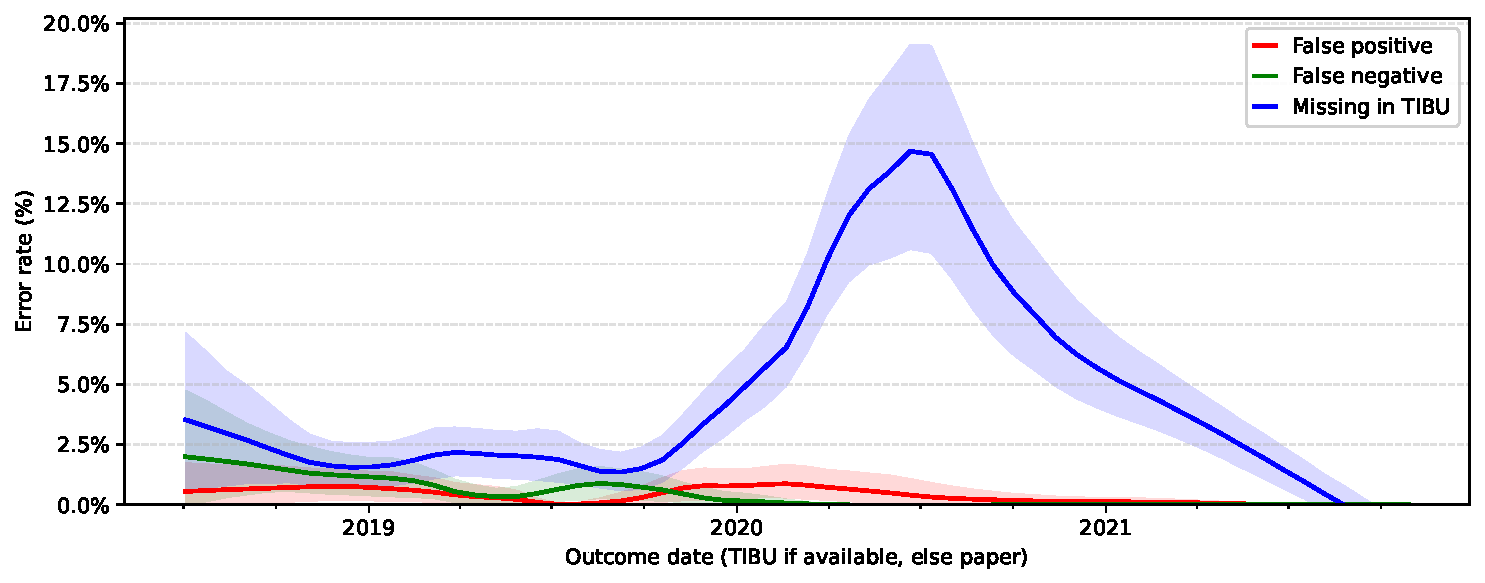
\includegraphics[width=0.85\textwidth]{fig_error_over_time_gated.pdf}
    \caption{DQA error rates over time, under the date-gated definition. Compare with Figure~\ref{fig:over_time}.}
    \label{fig:over_time_gated}
\end{figure}

% =============================================================================
\section{Multivariate predictors of missing-in-TIBU}
\label{sec:appendix_logit}
% =============================================================================

The marginal breakdowns in \S\S\ref{sec:errors_where} and \ref{sec:errors_who} stratify error rates one characteristic at a time, leaving open whether apparent associations reflect that characteristic or a correlated confound. Table~\ref{tbl:logit_errors} reports a logistic regression of missing-in-TIBU on individual, clinic, and record-age covariates jointly, with province fixed effects. We restrict to missing-in-TIBU because the false-positive and false-negative rates (31 and 21 events respectively) are too low to identify a multivariate model with province FE; the marginal evidence for those error types is in Tables~\ref{tbl:clinic_errors}--\ref{tbl:patient_errors}, and false positives are in any case dominated by audit-snapshot artifacts (\S\ref{sec:date_errors}). The first column uses the full classifiable sample; the second column excludes the two clinics responsible for the COVID-era reporting gap (clinic IDs 0 and 115, together $\approx 43\%$ of missing-in-TIBU events) as a sensitivity check, since events concentrated in those two clinics could otherwise drive coefficients on covariates merely correlated with their idiosyncratic profile.

\begin{table}[H]
    \centering
    \caption{Average marginal effects on the probability of missing-in-TIBU, in percentage points; cluster-robust standard errors (by clinic) in parentheses.}
    \label{tbl:logit_errors}
    {\footnotesize\begin{tabular}{l c c c c}
\toprule
 & \multicolumn{2}{c}{Missing in TIBU} & \multicolumn{2}{c}{False transfer} \\
\cmidrule(lr){2-3}\cmidrule(lr){4-5}
 & All & Excl.\ 0,\,115 & All & Excl.\ 162,\,50 \\
\midrule
\textit{Individual characteristics} & & & & \\
\quad Male & +2.79 & -0.21 & +2.17$^{**}$ & +1.85 \\
           & (1.91) & (0.51) & (0.72) & (1.02) \\
\addlinespace[3pt]
\quad Age (years) & -0.00 & -0.00 & -0.04 & -0.00 \\
           & (0.02) & (0.01) & (0.02) & (0.01) \\
\addlinespace[3pt]
\quad HIV positive & +0.17 & +0.03 & -1.15 & -1.91$^{***}$ \\
           & (0.62) & (0.31) & (1.39) & (0.56) \\
\addlinespace[3pt]
\quad Extrapulmonary TB & +1.01 & +0.82 & +0.82 & -0.54 \\
           & (0.92) & (0.61) & (0.67) & (0.75) \\
\addlinespace[3pt]
\quad Retreatment case & +0.09 & +0.07 & -1.46 & +0.17 \\
           & (0.81) & (0.87) & (2.07) & (0.83) \\
\addlinespace[3pt]
\quad Bacteriologically confirmed & +0.63 & +0.98$^{*}$ & +0.63 & +0.06 \\
           & (0.81) & (0.43) & (1.30) & (0.53) \\
\addlinespace[3pt]
\addlinespace[2pt]
\textit{Clinic characteristics} & & & & \\
\quad Urban clinic & +1.61 & +1.80 & +0.71 & +0.98 \\
           & (1.41) & (0.96) & (3.50) & (1.31) \\
\addlinespace[3pt]
\quad Clinic size (log patients) & -1.04 & +0.19 & +1.43$^{**}$ & -1.09 \\
           & (0.58) & (0.36) & (0.51) & (0.63) \\
\addlinespace[3pt]
\addlinespace[2pt]
\textit{Record characteristics} & & & & \\
\quad Record age (years) & -8.43$^{***}$ & -3.44$^{*}$ & -5.38$^{**}$ & -3.21 \\
           & (2.35) & (1.55) & (2.04) & (1.74) \\
\addlinespace[3pt]
\midrule
Province fixed effects & Yes & Yes & No & No \\
$N$ & 3,180 & 2,776 & 3,180 & 2,771 \\
Events & 86 & 28 & 130 & 44 \\
Clinics & 53 & 51 & 53 & 51 \\
McFadden's $R^2$ & 0.399 & 0.240 & 0.155 & 0.140 \\
\bottomrule
\addlinespace[3pt]
\multicolumn{5}{l}{\footnotesize \textit{Notes:} Cells report the average marginal effect on the probability of the} \\
\multicolumn{5}{l}{\footnotesize column outcome, in percentage points; cluster-robust standard errors (by clinic),} \\
\multicolumn{5}{l}{\footnotesize propagated to the AME via the delta method, are in parentheses below each estimate.} \\
\multicolumn{5}{l}{\footnotesize Province fixed effects (included but not displayed) are identified for missing-in-TIBU but} \\
\multicolumn{5}{l}{\footnotesize omitted for the sparser false-transfer outcome. Each ``Excl.'' column drops that outcome's two dominant clinics.} \\
\multicolumn{5}{l}{\footnotesize $^{***}p<0.001$,\ $^{**}p<0.01$,\ $^{*}p<0.05$.} \\
\end{tabular}}
\end{table}

Removing the two COVID clinics collapses both nominally interesting non-temporal coefficients. The point estimate on \emph{Male} moves from $+2.6$~pp to $-0.3$~pp, and the estimate on \emph{Clinic size} moves from $-1.0$~pp/log-patient to $+0.3$~pp; neither is statistically significant in either specification, but the full-sample estimates were suggestive enough to warrant the check. \emph{Record age} survives in both columns but its magnitude more than halves (from $-8.4$ to $-3.6$~pp/year, with significance falling from $p < 0.001$ to $p < 0.05$). We read this as a mostly mechanical reporting-lag effect: at any fixed snapshot date, more recent records have had less time to be transcribed into TIBU. The two COVID clinics inflate the slope because their missing-in-TIBU records cluster in the late, COVID-affected portion of the registration window. Outside those two clinics, neither patient demographics nor clinic-level structural features predict TIBU missingness in this sample; the only systematic signal is a modest record-age gradient consistent with reporting lag.

\end{document}
